\section{Storing Groceries [DSPL \& OPL]}

The robot must help put the newly bought groceries in the right place.
The owner of the robot will put the items on a table and the robot helps the owner by moving the groceries from a table to the right place in the cupboard.
What the right place for an item is defined by the objects already in the cupboard: objects of the same type must be placed together.
For example, the new pack of cookies from the table must be placed by the almost empty pack cookies in the cupboard.

In the cupboard and on the table, there will be both known, alike and unknown objects. 

\subsection{Goal}
The robot has to correctly identify and manipulate objects at different heights, grouping them by category and likelihood.

\subsection{Focus}
This test focuses on the detection and recognition of objects and their features, as well as object manipulation.

\subsection{Setup}
\begin{enumerate}
\item \textbf{Location:} One of the bookcases or cupboards in the apartment is used for this test, one where a table is near or can be put. 
The robot will start somewhere between the cupboard and the table. 
The cupboard has ca. 5 shelves between 0.30m and 1.80m from the ground. 
\item \textbf{Cupboard:} The cupboard contains 10 objects from the Scenario Objects \ref{rule:scenario_objects}. 
\item \textbf{Door:} The cupboard has a single door, which is closed initially.
The robot may ask a human to open the door, after which a referee will open the door. 
\item \textbf{Table:} 10 objects from the Scenario Objects \ref{rule:scenario_objects} will be placed on the table. If not all 10 objects fit the on the table, remaining objects can be added during the test.
\end{enumerate}

Please note that there may be more than one object in each shelf to fit all objects in, especially after the robot fills the shelves. 

\subsection{Task}
\textbf{Opening door:} The cupboard's door is closed and must be opened at some point in the challenge. Note that quickly opening the door also yields a small time advantage.
\begin{enumerate}
\item \textbf{Searching for objects:} The robot approaches the table from its nearby starting position and starts searching for objects. 
\item \textbf{Grasping objects:} Any object found on the table by the robot may be grasped by it. 
  Before or right after grasping the object, the robot may announce which object it has found. 
  % The scoring only takes the classifications in the report into account. 
\item \textbf{Placing objects:} After grasping the object, the robot has to safely place it (Section \refsec{rule:scenario_objects}) near the item of the same class in the cupboard. 
  The object must stay there for at least 10 seconds.
\item \textbf{Repeat:} This repeats until the time is up or all groceries are stored. 
\end{enumerate}

\subsection{Additional rules and remarks}
\begin{enumerate}
\item \textbf{Bypassing Manipulation:} Bypassing object manipulation via the CONTINUE rule (Section \refsec{rule:asrcontinue}) is not allowed during this test.
\item \textbf{No setup:} There is no setup time.
\item \textbf{Startup:} The robot must be started with a simple voice command or via a start button (Section \refsec{rule:start_signal}). 
\item \textbf{Single try:} The robot must be able to start from the first attempt. There is no restart for this test. If the robot is unable to start it must be removed immediately.
\item \textbf{Collisions:} Slightly touching the the cupboard is tolerated.
  Driving over the objects or any other form of a major collision is not allowed, and the referees directly stop the robot (Section \refsec{rule:safetyfirst}).
\item \textbf{Recognition report:} Robots must create a PDF report file including the list of recognized objects with a picture showing the object and the object name/label.
  This file may be stored on a USB-stick on the robot which is given to the TC after the test. The PDF file name should include the team name and a timestamp. 
  Furthermore, it must be unmistakable which label belongs to which object. Objects must also be recognizable in the report by a human (TC) so that it can be scored. 
  An overview of the shelf and/or table with bounding boxes and labels attached to the bounding boxes is handy for the TC to score.
  False positives in the report (labeling an object which is not an object but e.g. the edge of the shelf) are penalized.
%\item \textbf{QR Codes:} The team may request to use a special set ob objects identified with QR codes if the robot is not able to correctly recognize the objects. The use of this special QR-object-set must be announced to the TC at least on hour before the test starts. When QR Codes are used, no points are given for object recognition.
  \item \textbf{Clear area: } The robot may assume that the direct vicinity of the cupboard and table are clear and that the robot can move slightly backwards for its task.
  \item \textbf{Unknown objects:} A significant amount of objects are unknown objects. A correct label for these may be constituted by: 
  \begin{itemize}
   \item Simply labeling those as ``Unknown'' as opposed to wrongly applying a label from the known or alike objects
   \item Labeling pairs of unknown objects of the same class with the same label (which may be e.g. ``label0'' for one pair and ``label1'' for another). 
   \item Labeling unknown objects with a new, sensible label for objects.
  \end{itemize}
\end{enumerate}

\subsection{Data recording}
  Please record the following data (See \refsec{rule:datarecording}):
  \begin{itemize}
   \item Images
   \item Plans
  \end{itemize}

\subsection{OC instructions}

\textbf{2 hours before the test}
\begin{itemize}
    \item Anounce the startup location for robots.
\end{itemize}

\subsection{Referee instructions}
The referee needs to
\begin{itemize}
\item Place the objects in the cupboard and a few of the same class on the table. New items can be placed when there is room or the robot asks for more objects. 
\item Close the door of the cupboard. 
\item Put objects on the table and the corresponding objects in the cupboard: 3 known objects, 2 alike and 5 unknown objects. 
\end{itemize}

\begin{figure}
  \centering
  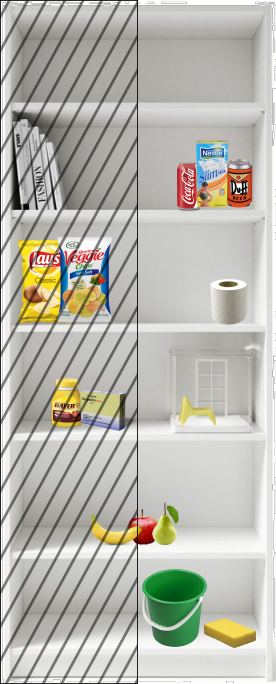
\includegraphics[width=0.25\textwidth]{images/storing_groceries.png}
  \vspace{-10pt}
  \label{fig:storing_groceries}
  \caption{Example shelf where objects will be placed.}
\end{figure}

\subsection{Score sheet}

The maximum time for this test is 3 minutes.

\begin{scorelist}
% There are 5 filled shelves
% On each shelf, there can fit 4 objects: 2 originally there, in the corners. As each object may get a 'companion' put there by the robot, there are 2 more objects per shelf.

% Grasp (any object): 10
% Place (anywhere in the cupboard): 10
% Place in correct place: 15
% Recognize known object correctly (without grasping/placing something of that class): 10
% Label two unknown objects of the same class with the same label (e.g. ``class0''): 15

% Place known object near known object of same class: 40
% Place unknown object near unknown object of the same class: 50


	\scoreheading{Grasping objects}
	\scoreitem[5]{10}{For each successful grasp of any object (lifting it up to at least 5 cm for more than 10 seconds)}

	\scoreheading{Placing objects}
	\scoreitem[5]{10}{For each successful placement of an object anywhere in the cupboard (safely stands still for more than 10 seconds)}
	\scoreitem[5]{5}{For each successful placement of an object at correct place (near an object of the same class)}

	\scoreheading{Recognizing objects}
	\scoreitem[5]{10}{Every correctly recognized known or alike object in the report file}
	\scoreitem[5]{15}{Corresponding labels for pairs of unknown objects of the same class, in the report file 
            \footnote{Suppose there is a rubber ducky as an unknown object class. Two rubber duckies must be given the same label (e.g. ``label0'') to receive these points}}
	\scoreitem[5]{-5}{False positive label}
	
% 	\scoreheading{Total task}
% 	\scoreitem[5]{40}{Place known object near known object of same class}
% 	\scoreitem[5]{50}{Place unknown object near unknown object of same class}

	\scoreheading{Bonus}
	\scoreitem[1]{20}{Open the door without human help}
	
	\setTotalScore{250}
\end{scorelist}


% Local Variables:
% TeX-master: "Rulebook"
% End:


% Local Variables:
% TeX-master: "Rulebook"
% End:
